\documentclass{article}
\usepackage[sglblindworkshop,final]{neurips_2026}
\workshoptitle{Vision-Language Models for Real-World Deployment (VLM4RWD), VistaQA Challenge Track 1}

\usepackage[utf8]{inputenc}
\usepackage[T1]{fontenc}
\usepackage[hidelinks]{hyperref}
\usepackage{url}
\usepackage{booktabs}
\usepackage{array}
\usepackage{amsmath}
\usepackage{microtype}
\usepackage{xcolor}
\usepackage{colortbl}
\definecolor{oursbg}{HTML}{E2ECFA}
\newcommand{\ours}{\rowcolor{oursbg}}
\usepackage{tikz}
\usepackage{graphicx}
\usetikzlibrary{positioning,arrows.meta,fit,shadows.blur}
\usepackage{listings}
\lstset{basicstyle=\ttfamily\scriptsize,breaklines=true,columns=fullflexible,frame=single}

\newcommand{\todo}[1]{\textcolor{red}{[#1]}}

\title{Grounding the Ungroundable:\\ Answers, Masks, and Absences in Zero-Shot VQA}

\author{Anonymous Authors}

\begin{document}
\maketitle

\begin{abstract}
A hallmark of a deployable vision-language system is the capacity to progress from answering a question about an image to
grounding that answer in pixels, and to recognize when the object asked about is not there. This capability, however,
remains fragile in current systems, which pair one vision-language model with a promptable segmenter and trust that model
alone to notice a false premise. Using VistaQA, where 27\% of questions ask about something absent, as a precise instrument,
we introduce a zero-shot chain of open-weight models that answers, grounds, and then doubts the premise: Qwen3.6-27B answers
and boxes its evidence, SAM3 turns the boxes into instance masks, a separate Qwen3-VL-8B pass checks whether the premise is
visible, and a guarded rule raises under-counted answers. Every choice was made on an external 560-question proxy, and the
configuration was registered before VistaQA was scored once. The entry scores \textbf{48.40 GROVE} with the AWQ build of
the paper's judge (\textbf{48.14} with the unquantized one), against 45.53 for the best published system (GPT-5.4-Thinking +
SAM3), with most of the margin from false-premise questions (70.9 vs 47.9). We also report what did not transfer: the count rule lost
0.55, partly through a bug found after scoring, and four later systems registered the same way scored 48.01 to 48.37. Our
findings expose a clear lesson for deployment: a grounded answering system gains most of its edge by recognizing when
there is nothing to ground.
\end{abstract}

\section{Introduction}
Grounded visual question answering remains a significant hurdle for vision-language models (VLMs). VistaQA~\cite{vistaqa}
asks a model to answer a free-form question about an image and to segment every instance of the evidence behind its answer.
The difficulty intensifies when the question itself is wrong: 27\% of its 1,157 questions have a false premise, and the right
response says the object is not there, with no masks, as a deployed assistant must. Because GROVE (Section~\ref{sec:setup})
caps a wrong answer at $0.1$ and gives such a response the full 1.0, answer accuracy and a reliable premise check matter more
than masks. Yet the strongest published systems pair one VLM with SAM3~\cite{sam3} and leave the premise to it alone, creating a gap between grounding what is asked and recognizing what cannot be grounded.

To bridge this gap, we separate three jobs (Fig.~\ref{fig:pipe}): a strong open VLM answers and boxes its evidence, a
promptable segmenter turns the boxes into masks, and a second VLM pass, which never sees the answer, checks the premise.
This paper's contributions are threefold: (1) We introduce an open-weight, training-free system that scores 48.40 GROVE on
VistaQA, against 45.53 for the best published system. (2) We adopt a zero-shot protocol in which every choice was made on
external proxy sets and every VistaQA run was registered before scoring. (3) Crucially, we show which dev-set gains
transferred: the premise check did, while most others did not.

\section{Related work}
\textbf{Grounded answering with masks.} Reasoning-segmentation models such as LISA~\cite{lisa}, GLaMM~\cite{glamm} and
Sa2VA~\cite{sa2va} train a VLM to emit segmentation tokens that a mask decoder turns into masks. On VistaQA the nine published
systems that do not use SAM3, these three among them, score 11.8 to 29.0 GROVE, while the five that pair a general VLM with SAM3 score 39.6 to 45.5
(Table~\ref{tab:main}). Our system belongs to the second, modular family, as does Grounded-SAM~\cite{groundedsam}: a VLM or
detector proposes boxes, and a promptable segmenter (SAM~\cite{sam}, SAM~2~\cite{sam2}, SAM3~\cite{sam3}) draws the masks.

\textbf{False premises and hallucination.} POPE~\cite{pope} measures object hallucination with yes/no questions about object
presence; we reuse its question form to confirm that an object is missing. SESAME~\cite{sesame} trains a multimodal model to
recognise and correct false premises before segmenting. We get similar behaviour without training, from a check asked only
what the question assumes and the image lacks.

\section{Methodology}\label{sec:system}
\begin{figure}[t]
\centering
% Figure 1: the entry's passes and merge rules, in the style of the team's diagrams/main-diagram.png, with the facts checked
% against src/pipeline.py and Scripts/fleet.py (remask -> override -> countfix). The scene is a synthetic illustration and
% the question is not a VistaQA question; box and mask are drawn over the photo in [0,1] image coordinates. The two logos
% are cut from main-diagram.png. Needs \usetikzlibrary{arrows.meta,shadows.blur}.
\definecolor{aTab}{HTML}{2D68AD}\definecolor{aLine}{HTML}{7DA4E0}\definecolor{aFill}{HTML}{EEF4FD}%
\definecolor{bTab}{HTML}{7E62B0}\definecolor{bLine}{HTML}{B9A1DE}\definecolor{bFill}{HTML}{F5EFFB}%
\definecolor{cTab}{HTML}{D9772F}\definecolor{cLine}{HTML}{EDAA78}\definecolor{cFill}{HTML}{FFF7EE}%
\definecolor{dTab}{HTML}{4A8F35}\definecolor{dLine}{HTML}{98C788}\definecolor{dFill}{HTML}{F3F9EE}%
\definecolor{vlmFill}{HTML}{E6EFFC}\definecolor{vlmLine}{HTML}{7DA4E3}\definecolor{samFill}{HTML}{EFE5FA}\definecolor{samLine}{HTML}{B094DD}%
\definecolor{outFill}{HTML}{EAF5E3}\definecolor{outLine}{HTML}{A6CF93}\definecolor{okg}{HTML}{3E8E24}%
\definecolor{mFill}{HTML}{F8F3FB}\definecolor{mLine}{HTML}{B9A3D9}\definecolor{mNum}{HTML}{8E73BD}\definecolor{oTab}{HTML}{1F4F8F}%
\definecolor{ink}{HTML}{1E1E1E}\definecolor{boxLine}{HTML}{C5CBD4}\definecolor{cardLine}{HTML}{D2D2D8}%
\definecolor{contFill}{HTML}{F7F9FC}\definecolor{contLine}{HTML}{D3DBE8}\definecolor{legFill}{HTML}{F7F7F9}\definecolor{boxred}{HTML}{E34948}%
\def\womanbox{(0.325,0.005) rectangle (0.655,0.675)}%
\def\womanmask{(0.480,0.667) -- (0.536,0.649) -- (0.569,0.589) -- (0.569,0.507) -- (0.559,0.444) -- (0.590,0.422) --
  (0.641,0.360) -- (0.648,0.056) -- (0.574,0.044) -- (0.572,0.005) -- (0.349,0.005) -- (0.331,0.111) -- (0.336,0.211) --
  (0.356,0.356) -- (0.389,0.433) -- (0.402,0.533) -- (0.426,0.633) -- cycle}%
\protected\def\nohy{\hyphenpenalty=10000\relax}%
\newsavebox\scIn\newsavebox\scBox\newsavebox\scBoxB\newsavebox\scMask\newsavebox\scOut%
\newsavebox\icBox\newsavebox\icGear\newsavebox\icCheck\newsavebox\icRefresh%
\newcommand{\scene}[3]{\sbox#1{\begin{tikzpicture}
  \node[anchor=south west, inner sep=0] (im) at (0,0) {
\includegraphics[width=#2]{diagrams/scene.png}};
  \begin{scope}[x={(im.south east)}, y={(im.north west)}] #3 \end{scope}\end{tikzpicture}}}%
\scene\scIn{1.75cm}{}%
\scene\scBox{1.17cm}{\draw[boxred, line width=0.7pt] \womanbox;}%
\scene\scBoxB{0.9cm}{\draw[boxred, line width=0.6pt] \womanbox;}%
\scene\scMask{0.9cm}{\fill[black] (0,0) rectangle (1,1); \fill[white] \womanmask;}%
\scene\scOut{1.55cm}{\fill[black] (0,0) rectangle (1,1); \fill[white] \womanmask;}%
\sbox\icBox{\tikz[baseline=-0.6ex]\draw[rounded corners=0.6pt, line width=0.4pt] (0,-0.065) rectangle (0.13,0.065);}%
\sbox\icGear{\tikz[baseline=-0.6ex]{\foreach \a in {0,45,...,315} \fill[ink, rotate=\a] (-0.026,0.06) rectangle (0.026,0.1);
  \fill[ink] (0,0) circle (0.075); \fill[white] (0,0) circle (0.042); \draw[ink, line width=0.35pt] (0,0) circle (0.022);}}%
\sbox\icCheck{\tikz[baseline=-0.5ex]\draw[white, line width=0.9pt, line cap=round, line join=round] (0,0.01) -- (0.045,-0.04) -- (0.13,0.065);}%
\sbox\icRefresh{\tikz[baseline=-0.6ex]\draw[bTab, line width=0.5pt, -{Stealth[length=0.75mm, width=0.9mm]}] (70:0.07) arc (70:340:0.07);}%
\newcommand\chipt[4]{$\vcenter{\hbox{\includegraphics[height=#2]{diagrams/logo_#1}}}$\hspace{3pt}%
  $\vcenter{\hbox{\def\arraystretch{0.92}\begin{tabular}{@{}l@{}}\textbf{#3}\\#4\end{tabular}}}$}%
%
% rows: A -0.2/-1.42, B -1.57/-2.52, C -2.67/-3.82, D -3.97/-5.36; container 0/-5.45; panels x 2.38..9.27
\begin{tikzpicture}[font=\sffamily\fontsize{6}{7}\selectfont\nohy, line join=round,
  sh/.style={blur shadow={shadow blur steps=6, shadow xshift=0.3pt, shadow yshift=-0.6pt, shadow blur radius=1.4pt, shadow opacity=20}},
  panel/.style 2 args={draw=#1, fill=#2, rounded corners=4pt, line width=0.7pt, sh},
  pill/.style={fill=#1, text=white, font=\sffamily\bfseries\fontsize{6.3}{7}\selectfont, rounded corners=1.6mm,
    inner xsep=4pt, inner ysep=1.5pt, minimum height=0.32cm, anchor=west, sh},
  chip/.style 2 args={draw=#1, fill=#2, rounded corners=3pt, line width=0.55pt, minimum width=1.9cm, minimum height=0.6cm, inner sep=1.5pt, sh},
  vlm/.style={chip={vlmLine}{vlmFill}}, sam/.style={chip={samLine}{samFill}},
  wbox/.style={draw=boxLine, fill=white, rounded corners=3pt, line width=0.45pt, inner sep=2.2pt, align=flush left},
  gbox/.style={draw=outLine, fill=outFill, rounded corners=3pt, line width=0.45pt, inner sep=2.2pt, align=flush left},
  arr/.style={-{Stealth[length=1.5mm, width=1.15mm]}, line width=0.55pt, draw=ink},
  numc/.style={circle, fill=mNum, text=white, font=\sffamily\bfseries\fontsize{5.6}{6}\selectfont, inner sep=0pt, minimum size=0.27cm},
  rule/.style={anchor=north west, text width=1.75cm, inner sep=0, align=flush left},
  leg/.style={anchor=west, inner sep=0, font=\sffamily\fontsize{5.3}{6}\selectfont}]
\useasboundingbox (-0.02,0.05) rectangle (13.95,-5.55);

% ---- input card ----
\draw[fill=white, draw=cardLine, rounded corners=4pt, line width=0.5pt, sh] (0,0) rectangle (1.95,-3.27);
\node[inner sep=0] at (0.975,-0.78) {\usebox\scIn};
\node at (0.975,-1.57) {\itshape Image $\boldsymbol{x}$};
\draw[fill=legFill, draw=cardLine, rounded corners=3pt, line width=0.45pt] (0.1,-1.75) rectangle (1.85,-3.15);
\node[fill=bTab, text=white, rounded corners=1.2pt, inner sep=0pt, minimum size=0.25cm, font=\sffamily\bfseries\fontsize{5.6}{6}\selectfont] at (0.29,-1.95) {Q};
\node[anchor=west, inner sep=0, font=\sffamily\bfseries\fontsize{6.3}{7}\selectfont] at (0.47,-1.95) {Question $\boldsymbol{q}$};
\node[anchor=north west, inner sep=0, text width=1.6cm, align=flush left, font=\sffamily\itshape\fontsize{6}{7}\selectfont\nohy] at (0.17,-2.15) {Which person is carrying a shopping bag?};

% ---- legend card ----
\draw[fill=legFill, draw=cardLine, rounded corners=4pt, line width=0.5pt, sh] (0,-3.42) rectangle (1.95,-5.45);
\node[anchor=west, inner sep=0, font=\sffamily\bfseries\fontsize{6.3}{7}\selectfont] at (0.12,-3.64) {Legend};
\draw[arr] (0.1,-3.92) -- (0.36,-3.92); \node[leg] at (0.43,-3.92) {data flow};
\draw[arr, dashed, draw=bTab] (0.1,-4.22) -- (0.36,-4.22); \node[leg] at (0.43,-4.22) {conditional};
\draw[fill=vlmFill, draw=vlmLine, rounded corners=1.5pt, line width=0.45pt] (0.1,-4.6) rectangle (0.36,-4.44); \node[leg] at (0.43,-4.52) {VLM (Qwen)};
\draw[fill=samFill, draw=samLine, rounded corners=1.5pt, line width=0.45pt] (0.1,-4.9) rectangle (0.36,-4.74); \node[leg] at (0.43,-4.82) {SAM3 segmenter};
\draw[fill=outFill, draw=outLine, rounded corners=1.5pt, line width=0.45pt] (0.1,-5.2) rectangle (0.36,-5.04); \node[leg] at (0.43,-5.12) {Model output};

% ---- container and the four passes ----
\draw[fill=contFill, draw=contLine, rounded corners=5pt, line width=0.5pt, sh] (2.27,0) rectangle (9.38,-5.45);
\draw[panel={aLine}{aFill}] (2.38,-0.2) rectangle (9.27,-1.42);
\draw[panel={bLine}{bFill}] (2.38,-1.57) rectangle (9.27,-2.52);
\draw[panel={cLine}{cFill}] (2.38,-2.67) rectangle (9.27,-3.82);
\draw[panel={dLine}{dFill}] (2.38,-3.97) rectangle (9.27,-5.36);
\node[pill=aTab] at (2.48,-0.2) {A. Answer and evidence boxes};
\node[pill=bTab] at (2.48,-1.57) {B. Masks from boxes};
\node[pill=cTab] at (2.48,-2.67) {C. Premise check (answer-agnostic)};
\node[pill=dTab] at (2.48,-3.97) {D. Counters (plain counting questions)};

% bus from the input to every pass; D runs only on counting questions
\draw[line width=0.55pt, draw=ink] (1.95,-2.45) -- (2.12,-2.45);
\draw[line width=0.55pt, draw=ink] (2.12,-0.7) -- (2.12,-3.28);
\foreach \y in {-0.7,-2.1,-3.28} \draw[arr] (2.12,\y) -- (2.38,\y);
\draw[arr, dashed, draw=dTab] (2.12,-3.28) -- (2.12,-4.75) -- (2.38,-4.75);

% A
\node[vlm] (a) at (3.45,-0.68) {\chipt{qwen}{0.3cm}{Qwen3.6-27B}{(NF4, 4-bit)}};
\node[draw=bTab, dashed, fill=bFill, rounded corners=1.4mm, line width=0.5pt, inner xsep=2.5pt, inner ysep=1.2pt,
  font=\sffamily\fontsize{5.2}{6}\selectfont] (rw) at (3.5,-1.18) {\usebox\icRefresh\hspace{2pt}\textbf{Rewrite} if $\leq$3 words};
\node[wbox, text width=2.95cm] (aout) at (6.2,-0.86) {\textbf{Answer:} \emph{The woman in front is carrying a red bag.}\\[1pt]
  \textbf{Boxes:} \usebox\icBox\ $[x_1, y_1, x_2, y_2]$ \dots};
\node[inner sep=0] (athumb) at (8.565,-0.86) {\usebox\scBox};
\draw[arr] (a.east) -- (a.east -| aout.west);
\draw[arr] (aout) -- (athumb);

% B
\node[sam] (b) at (3.45,-2.1) {\chipt{sam3}{0.24cm}{SAM3}{(box prompts)}};
\node[inner sep=0] (bbox) at (5.42,-2.1) {\usebox\scBoxB};
\node[inner sep=0] (bmask) at (6.57,-2.1) {\usebox\scMask};
\node[wbox, text width=1.8cm, align=center] (bout) at (8.21,-2.1) {One mask per box\\(full resolution)};
\draw[arr] (b) -- (bbox); \draw[arr] (bbox) -- (bmask); \draw[arr] (bmask) -- (bout);
\draw[arr, draw=bTab] (aout.south -| bbox) -- (bbox.north);

% C
\node[vlm] (c) at (3.45,-3.28) {\chipt{qwen}{0.3cm}{Qwen3-VL-8B}{(fp16)}};
\node[wbox, text width=3.0cm, font=\sffamily\fontsize{5.5}{6.4}\selectfont\nohy] (cout) at (6.22,-3.31) {\textbf{Task:} Name any \emph{X} the
  question assumes but the image lacks, then ask: \emph{Is there any X in the image?}};
\node[gbox, align=center, text width=0.95cm] (cres) at (8.62,-3.31) {\textbf{Missing:}\\\textcolor{okg}{\textbf{none}}};
\draw[arr] (c) -- (cout); \draw[arr] (cout) -- (cres);

% D
\node[sam, inner ysep=0.8pt] (d1) at (3.45,-4.44) {\chipt{sam3}{0.24cm}{SAM3}{(text prompt)}};
\node[vlm, inner ysep=0.8pt] (d2) at (3.45,-5.04) {\chipt{qwen}{0.3cm}{Qwen3-VL-8B}{(fp16)}};
\node[gbox, text width=1.8cm] (g1) at (5.72,-4.44) {\textbf{Label} from \textbf{A}\\(score $\geq$ 0.8)};
\node[gbox, text width=1.8cm] (g2) at (5.72,-5.04) {\textbf{Count from VLM}};
\node[draw=ink, fill=white, rounded corners=2.5pt, line width=0.55pt, inner sep=2pt] (mx) at (7.42,-4.74) {max};
\node[gbox, text width=1.05cm] (g3) at (8.62,-4.74) {\textbf{Counter:} only raises A's count};
\draw[arr] (d1) -- (g1); \draw[arr] (d2) -- (g2);
\draw[arr, rounded corners=2pt] (g1.east) -- ++(0.17,0) |- ([yshift=1.2pt]mx.west);
\draw[arr, rounded corners=2pt] (g2.east) -- ++(0.17,0) |- ([yshift=-1.2pt]mx.west);
\draw[arr] (mx) -- (g3);

% ---- rule-based merge ----
\draw[panel={mLine}{mFill}] (9.62,-0.6) rectangle (11.88,-4.85);
\begin{scope}\clip[rounded corners=4pt] (9.62,-0.6) rectangle (11.88,-4.85); \fill[white] (9.62,-0.6) rectangle (11.88,-1.05); \end{scope}
\draw[mLine, line width=0.7pt, rounded corners=4pt] (9.62,-0.6) rectangle (11.88,-4.85);
\draw[mLine, line width=0.4pt] (9.62,-1.05) -- (11.88,-1.05);
\node[anchor=west, inner sep=0, font=\sffamily\bfseries\fontsize{6}{7}\selectfont] at (9.72,-0.825) {\usebox\icGear\hspace{3pt}Rule-based Merge};
\node[numc] at (9.84,-1.3) {1}; \node[rule] at (10.03,-1.2) {Attach \textbf{B}'s masks to \textbf{A}'s answer, one per box.};
\draw[mLine, line width=0.35pt] (9.75,-2.0) -- (11.75,-2.0);
\node[numc] at (9.84,-2.25) {2}; \node[rule] at (10.03,-2.15) {If \textbf{C} names \emph{X} and \emph{Is there any X?} gets
  \textbf{no}: answer = ``There is no X in the image.'', masks~=~$\emptyset$.};
\draw[mLine, line width=0.35pt] (9.75,-3.62) -- (11.75,-3.62);
\node[numc] at (9.84,-3.87) {3}; \node[rule] at (10.03,-3.77) {If a plain counting question: raise \textbf{A}'s count to the
  larger counter from \textbf{D}.};
\draw[arr, draw=aTab, rounded corners=2pt] (9.27,-0.86) -- (9.47,-0.86) |- (9.62,-1.38);
\draw[arr, draw=bTab, rounded corners=2pt] (9.27,-2.1) -- (9.52,-2.1) |- (9.62,-1.62);
\draw[arr, draw=cTab] (9.27,-3.0) -- (9.62,-3.0);
\draw[arr, draw=dTab, rounded corners=2pt] (9.27,-4.75) -- (9.47,-4.75) |- (9.62,-4.15);

% ---- final output ----
\draw[arr] (11.88,-2.5) -- (12.1,-2.5);
\draw[draw=oTab, fill=white, rounded corners=4pt, line width=0.8pt, sh] (12.1,-0.85) rectangle (13.92,-4.1);
\node[pill=oTab, anchor=center, minimum width=1.68cm] at (13.01,-0.85) {\usebox\icCheck\hspace{3pt}Final Output};
\node[anchor=west, inner sep=0, font=\sffamily\bfseries\fontsize{6.3}{7}\selectfont] at (12.2,-1.25) {Answer:};
\node[gbox, text width=1.5cm, font=\sffamily\itshape\fontsize{6}{7}\selectfont\nohy] at (13.01,-2.0) {The woman in front is carrying a red bag.};
\node[anchor=west, inner sep=0, font=\sffamily\bfseries\fontsize{6.3}{7}\selectfont] at (12.2,-2.72) {Masks:};
\node[inner sep=0] at (13.01,-3.42) {\usebox\scOut};
\end{tikzpicture}%

\caption{Passes A--D run independently; fixed rules merge their outputs. The example is illustrative (synthetic image,
question not from VistaQA): C finds nothing missing and D does not apply.}
\label{fig:pipe}
\end{figure}

\textbf{A. Answer and evidence boxes.} Qwen3.6-27B~\cite{qwen3}, quantized to 4-bit NF4, gets one
prompt (App.~\ref{app:prompts}): answer in one short complete sentence, then list every object the answer rests on, one box per
instance, with ``one box per counted object'' and ``box the text you read'' as task hints and an empty list for unanswerable
questions. Images are capped at $1280^2$ pixels. Answers of three words or fewer are rewritten into a full sentence by the
same model, since the official judge rejects bare answers such as ``bed'' as incomplete.

\textbf{B. Masks.} Each box prompts the SAM3~\cite{sam3} tracker head and gives one mask at full image resolution. On the proxy
SAM3 and SAM2.1-L tied with the same boxes (71.72 vs 71.74); we kept SAM3 because the same model also gives the text-prompted
counts of pass D.

\textbf{C. Premise check.} Qwen3-VL-8B~\cite{qwen3vl} sees the image and question and is told not to answer but to name
any object, person, text or detail the question assumes and the image does not show. A named item is confirmed with a POPE-style
question~\cite{pope} (``Is there any X in the image? Answer yes or no''); on ``no'' the answer becomes ``There is no X in the
image.'' with no masks. The smaller model was a measured choice: for similar recall, the 27B raised more false alarms
on the proxy (36 vs 17).

\textbf{D. Count raise.} All our counters under-count. On plain counting questions (a regex for ``how many / count / number
of'' without arithmetic or conditions, at most 12 words), the 27B count may be raised to the number of SAM3 text-prompt
instances with score $\geq0.8$ (prompt = the 27B's evidence label) or to the 8B's count, whichever is larger; the masks of the
winning counter are used. The guard comes from a MathVista~\cite{mathvista} count probe, where raising on ``subtract all X''
or statistics questions broke more answers than it fixed.

\section{Experimental setup}\label{sec:setup}
\textbf{Benchmark and metric.} GROVE scores each VistaQA sample as $\sqrt{\max(T,\epsilon)\max(S,\epsilon)}$ with
$\epsilon=0.01$, where $T\in\{0,1\}$ is an LLM-judge verdict and $S$ the Hungarian-matched IoU sum divided by
$\max(\#\text{GT},\#\text{pred})$, and averages over samples. The paper's judge is Qwen2.5-14B-Instruct~\cite{qwen25}. Our
pre-registered scoring used its AWQ build with the official prompt and parser; a re-judging with the unquantized model, registered
before it ran, is reported alongside, and 48.40 remains the entry's score. Differences come with paired bootstrap 95\% CIs over samples.

\textbf{Zero-shot protocol and development data.} VistaQA was used once, for the final score. Every choice above---backbone, prompts, image size, segmenter, thresholds, merge
order---was made on an external \textbf{proxy dev} set of 560 templated questions with masks, built from COCO
val2017~\cite{coco} (counting, identification, spatial, comparison), PACO-LVIS~\cite{paco} (attributes) and COCO-Text
v2~\cite{cocotext} (OCR), with 150 false-premise questions (26.8\%). Two text-only probes covered what COCO cannot: MathVista
testmini for premises and counts on figures, TextVQA~\cite{textvqa} for reading. The frozen configuration scored 73.81 on the
proxy. It was registered in version control before VistaQA was scored, and the VistaQA predictions before they were
judged. At inference each pass reads only the image and the question. The evaluation harness was checked before any system was
scored (Appendix~\ref{app:judge}). The only change after freezing was a format fix: two VistaQA images are smaller than their JSON
declares, and three masks were resized to the declared size.

\textbf{Implementation.} Decoding is greedy throughout. Re-running 150 random VistaQA samples on a different
machine reproduced 147 answers exactly, and SAM3's 259 masks on the same boxes agree with mean IoU 0.9998. Prompts, constants,
checkpoints and merge order are in Appendices~\ref{app:prompts}--\ref{app:repro}.

\textbf{External resources.} Qwen3.6-27B, Qwen3-VL-8B-Instruct and the judge Qwen2.5-14B-Instruct(-AWQ) (Apache-2.0); SAM3
(SAM License; loaded from public mirrors whose SHA-256 matches the official release); bitsandbytes, vLLM, transformers.
Development data: COCO val2017, PACO-LVIS, COCO-Text v2, MathVista testmini, TextVQA val; for proxy2, BDD100K, BOP (YCB-V,
LM-O) and the 2018 Data Science Bowl. No training, fine-tuning or retrieval. Models and data used only in development or in
the post-freeze analyses are listed in Appendix~\ref{app:repro}.

\begin{table}[t]
\centering\scriptsize
\setlength{\tabcolsep}{2.2pt}
\caption{GROVE on VistaQA: the 14 published systems (quoted from the VistaQA paper, not re-run; the first five pair the named
VLM with SAM3) and our entry (shaded). The benchmark's judge is the unquantized Qwen2.5-14B-Instruct, so our full-judge row is
the like-for-like comparison; the AWQ row is our registered score. Gr.: grounded, FP: false-premise questions. Bold: best in each column.}
\label{tab:main}
\begin{tabular}{@{}lrrrrrrrrrrrrrrr@{}}
\toprule
 & & \multicolumn{6}{c}{Task} & \multicolumn{2}{c}{Question} & \multicolumn{6}{c}{Domain} \\
\cmidrule(lr){3-8}\cmidrule(lr){9-10}\cmidrule(l){11-16}
System & All & Ident. & Attr. & OCR & Spat. & Count & Comp. & Gr. & FP & Indoor & Outd. & Math & AV & Robot. & Sci. \\
\midrule
GPT-5.4-Thinking & 45.53 & \textbf{53.62} & 44.73 & 44.16 & 38.86 & \textbf{52.21} & 38.93 & \textbf{44.65} & 47.89 & 45.39 & 45.92 & \textbf{41.51} & 53.18 & \textbf{47.01} & 39.24 \\
Qwen3-VL-4B & 43.30 & 50.36 & 47.46 & 40.96 & 36.32 & 45.52 & 38.43 & 36.81 & 60.72 & 43.64 & 46.84 & 27.37 & 59.39 & 41.78 & 36.80 \\
Qwen3-VL-32B & 42.72 & 48.41 & 46.37 & 42.14 & 35.91 & 45.72 & 37.41 & 37.63 & 56.41 & 44.27 & 47.63 & 23.23 & 58.40 & 40.09 & 37.85 \\
GPT-5.4 & 41.50 & 48.22 & 40.43 & 41.33 & 35.62 & 47.06 & 35.86 & 43.28 & 36.72 & 42.06 & 46.05 & 28.99 & 53.43 & 39.87 & 35.54 \\
Gemini 3 & 39.63 & 43.10 & 40.11 & 42.55 & 33.53 & 42.81 & 35.84 & 33.48 & 56.14 & 39.37 & 39.40 & 31.40 & 48.42 & 37.15 & 39.87 \\
VRT-RL & 29.02 & 34.92 & 28.74 & 27.43 & 24.44 & 29.94 & 28.01 & 32.09 & 20.79 & 29.61 & 33.06 & 24.68 & 30.76 & 27.74 & 27.27 \\
Sa2VA-8B & 25.74 & 26.79 & 30.44 & 25.36 & 22.87 & 20.46 & 28.36 & 31.01 & 11.58 & 22.64 & 24.03 & 14.87 & 36.87 & 25.10 & 28.09 \\
UniPixel-7B & 22.39 & 22.24 & 28.29 & 22.19 & 19.90 & 15.36 & 26.34 & 25.98 & 12.75 & 21.76 & 23.20 & 12.90 & 28.87 & 21.02 & 24.15 \\
TreeVGR-7B & 19.03 & 18.28 & 18.55 & 16.42 & 17.90 & 20.25 & 22.65 & 17.68 & 22.66 & 18.41 & 20.45 & 12.70 & 23.51 & 19.76 & 17.78 \\
SESAME-7B & 17.02 & 17.90 & 17.14 & 13.62 & 18.48 & 17.60 & 16.90 & 12.17 & 30.04 & 17.20 & 17.68 & 11.05 & 20.77 & 15.92 & 17.97 \\
LISA-7B & 15.47 & 15.16 & 16.92 & 12.44 & 15.29 & 16.56 & 16.23 & 14.01 & 19.39 & 16.01 & 16.41 & 12.15 & 16.50 & 15.97 & 14.95 \\
GLaMM-7B & 13.53 & 14.86 & 12.89 & 12.34 & 14.19 & 11.84 & 14.70 & 14.48 & 10.96 & 12.82 & 13.75 & 11.13 & 15.70 & 13.43 & 13.72 \\
LaSagnA-7B & 12.35 & 13.31 & 12.03 & 11.04 & 13.23 & 11.14 & 13.05 & 13.12 & 10.28 & 11.31 & 12.18 & 11.07 & 14.05 & 12.09 & 13.07 \\
Uground-7B & 11.78 & 10.95 & 11.69 & 11.15 & 11.57 & 12.15 & 13.22 & 10.94 & 14.03 & 11.32 & 10.74 & 10.78 & 11.79 & 13.40 & 12.38 \\
\midrule
\ours Ours, AWQ judge & \textbf{48.40} & 50.77 & 52.61 & \textbf{58.37} & \textbf{41.75} & 44.57 & 43.24 & 40.03 & \textbf{70.88} & \textbf{54.09} & 55.65 & 26.14 & 67.55 & 32.60 & \textbf{48.63} \\
\ours Ours, full judge & 48.14 & 51.37 & \textbf{53.23} & 57.39 & 40.62 & 42.13 & \textbf{44.84} & 41.19 & 66.81 & 53.35 & \textbf{55.73} & 27.80 & \textbf{68.42} & 30.15 & 48.15 \\
\bottomrule
\end{tabular}
\end{table}

\section{Experiments and results}\label{sec:results}
\textbf{Comparison with published systems.} Table~\ref{tab:main} places the entry on the published board. It ranks first overall under both judges (95\% bootstrap
interval 45.95--50.90 with the AWQ judge) and first in 9 of the 14 task, question-type and domain columns. The lead comes from
false-premise questions. The entry is second on identification, third on grounded questions, fifth on counting and math (sixth
and fourth with the full judge) and sixth on robotics, where GPT-5.4-Thinking is far ahead (math 41.5 vs 26.1, robotics 47.0 vs
32.6). Text accuracy is level with that system (60.76 vs 61.02) but built differently: 72.0\% vs 39.2\% on false-premise
questions and 56.6\% vs 69.2\% on grounded ones. Our masks are better (mIoU 52.05 vs 41.98), which is what box-prompted SAM3 on a
strong localiser buys. The published systems' per-sample outputs are unreleased, so no comparison is paired.

\begin{table}[t]
\centering\small
\caption{Ablation, GROVE of each stage (the entry shaded). Proxy dev drove every decision; the VistaQA scores of the first two
rows were computed after freezing and are analysis only.}
\label{tab:abl}
\begin{tabular}{lrrrr}
\toprule
System & Proxy dev & VistaQA (AWQ) & VistaQA (full) & Text (AWQ) \\
\midrule
A + B: answer, boxes, SAM3 masks & 65.07 & 45.46 & 45.85 & 59.55 \\
+ C: premise check & 72.27 & 48.95 & 48.62 & 61.45 \\
\ours + D: count raise (\textbf{entry}) & 73.81 & \textbf{48.40} & \textbf{48.14} & 60.76 \\
\bottomrule
\end{tabular}
\end{table}

\textbf{Premise check (+3.49, 95\% CI +1.65 to +5.35).} Table~\ref{tab:abl} adds the passes one at a time, and this one gave
most of the gain. It caught 222 of 314 false-premise questions and fired on 110 of 843
grounded ones (13\%; 4\% on the proxy). False-premise GROVE rose from 45.7 to 70.9 and grounded GROVE fell from 45.4 to 40.8.

\textbf{Count raise ($-0.55$, CI $-1.02$ to $-0.13$).} It added 1.5 on the proxy and lost on VistaQA: of 23 raised answers, 10
went from right to wrong and 2 from wrong to right. After scoring we found a bug in the frozen entry: the 8B count pass
ran without masks, and the rule takes the winning counter's masks, so 11 of the 23 raised answers were left with none. The
proxy could not show this because its 8B pass had masks. The entry is unchanged; the same merge with masks kept (same answers,
registered as analysis) scores 48.47, so the bug cost 0.07; the rest of the loss is wrongly raised counts.

\textbf{Where the points go.} Of 51.6 GROVE points lost, 30.4 come from wrong answers to grounded questions, 11.9 from imperfect
masks on right answers, 7.3 from wrong answers to false-premise questions and 1.9 from missing or superfluous masks. Of 460 right
grounded answers with masks, 169 have more masks than the ground truth (mean $S$ 0.33 vs 0.74 with the exact count);
the proxy had one such case. Appendix~\ref{app:mv} tests a Set-of-Mark fix.

\section{Discussion and limitations}\label{sec:disc}
\textbf{Dev-set gains after the freeze mostly did not transfer.} The entry's aggregates (premise false alarms, over-masking,
weak math and robotics) prompted four later systems, each chosen on dev sets without looking at any VistaQA sample and
registered before its one VistaQA run (Appendix~\ref{app:v2}). For them we added \textbf{proxy2}, 580 questions on drawn charts,
tabletop object scenes~\cite{bop23,posecnn,lmo}, cell nuclei~\cite{dsb2018} and driving images~\cite{bdd100k}. v2 brought in
Qwen3.8-27B~\cite{qwen38}, a figure-specific evidence prompt and a SAM3 check that can overrule the premise check; v3 added
thinking on multi-step questions, v4 a calculator and v5 larger input images. v2 gained 8.4 on proxy2, yet all four scored 48.01
to 48.37 on VistaQA, within 0.4 of the entry: the dev sets predicted the premise check's gain but not the effect of the backbone
or the figure prompt.

\textbf{Limitations.} The system is weakest on math and robotics, where it trails GPT-5.4-Thinking by 15 and 14 points; thinking
and a calculator, tried after the freeze, did not close the math gap. The premise check trades grounded accuracy for
false-premise accuracy, and the count raise, chosen on templated proxy counts, lost on VistaQA. The COCO-based proxy understated
the check's false alarms (4\% vs 13\% of grounded questions) and showed almost no over-masking. We scored 22 systems on VistaQA without correcting the
intervals for that number; only the entry was frozen before VistaQA was scored.

\section{Conclusion}
A training-free chain of open-weight models, developed without VistaQA, scores 48.40 GROVE, ahead of the 14 published systems.
Most of the margin comes from false-premise questions, caught by a premise check that runs apart from the answerer. Code,
configurations, the run log with every registration, the predictions and their official evaluation:
\url{anonymized-repository-link} (checkpoints and merge order: Appendix~\ref{app:repro}).

\bibliographystyle{plain}
\bibliography{refs}

\appendix
\noindent\textbf{Guide to the appendices.} Appendices~\ref{app:prompts}--\ref{app:repro} specify the entry: prompts,
implementation constants, checkpoints and merge order. Appendix~\ref{app:qual} shows qualitative examples, \ref{app:anat} breaks the
entry's score down, \ref{app:judge} checks the judge and the evaluation harness, and \ref{app:dev} records every development
decision. Appendix~\ref{app:v2} details the four later systems of Section~\ref{sec:disc}, \ref{app:wsp}--\ref{app:ms} are
three further tests run after development closed, and \ref{app:transfer} compares dev-set and VistaQA effects across all changes. None of this changed the entry. Once the entry was scored, its VistaQA aggregates
did shape what we tried next, but every later choice was made on dev sets and every VistaQA run was registered before it ran. In
all we scored 22 systems on VistaQA; the run log lists them, and the intervals below are not corrected for that number. Unless
stated otherwise, scores use the AWQ judge and intervals are paired bootstrap 95\% CIs over samples (10,000 resamples, seed 0);
a few earlier values in the run log differ from these by up to 0.06. Wherever our entry appears in a table, it is shaded and
listed last.

\section{Prompts}\label{app:prompts}
\textbf{Pass A (answer + evidence).}
\begin{lstlisting}
You are given an image and a question about it.
1. Answer the question accurately and concisely, as one short complete sentence.
2. Localize the visual evidence: every object or region in the image that your answer is based on, one entry per object instance, each with a bounding box [x1, y1, x2, y2] in coordinates normalized to 0-1000.
- If you count objects, give one box per counted object; the number of boxes must equal your count.
- For questions about text, box the text region you read.
- If the object or entity the question asks about does not exist in the image, or the question cannot be answered from the image, say so in the answer and return an empty evidence list.

Question: {question}

Return only JSON: {"answer": "...", "evidence": [{"label": "...", "bbox_2d": [x1, y1, x2, y2]}]}
\end{lstlisting}
\textbf{Short-answer rewrite.}
\begin{lstlisting}
Question: {question}
Short answer: {answer}
Rewrite the short answer as one complete sentence that restates what the question asks about. Do not add or change any information. Return only the sentence.
\end{lstlisting}
\textbf{Pass C (premise) and confirm.}
\begin{lstlisting}
Question about this image: {question}
Do not answer the question. Check its premise: does the question assume an object, person, text or detail that is not actually visible in the image? Look carefully at the whole image.
If something it assumes is missing, name it in a few words; otherwise answer none.
Return only JSON: {"missing": "..."}

Is there any {missing} in the image? Answer yes or no.
\end{lstlisting}

\textbf{Appendix~\ref{app:v2}: figure router (Qwen3-VL-8B), reasoning router (Qwen3.8, no thinking).}
\begin{lstlisting}
Is this image a chart, plot, table, diagram or geometric figure, rather than a photograph or a rendering of a real scene? Answer yes or no.

Question about this image: {question}
Do not answer it. Does answering it need several steps of calculation or reasoning (arithmetic, algebra, geometry, physics, a logic puzzle), rather than reading a value, label or count directly from the image? Answer yes or no.
\end{lstlisting}
\textbf{Appendix~\ref{app:v2}: evidence prompt for routed figures} (Pass A with step 2 replaced by these lines).
\begin{lstlisting}
2. Localize the visual evidence: only what directly shows the answer, one entry per object instance, each with a bounding box [x1, y1, x2, y2] in coordinates normalized to 0-1000.
- Box the answer element itself, not what you read to find it: the bar or slice rather than its label or the legend, the table cell holding the value rather than its row and column headers, the shape rather than its side lengths.
- If the question compares or relates objects, box each of them.
\end{lstlisting}

\section{Implementation details}\label{app:impl}
\textbf{Data access.} The loader keeps only the image id, width, height and question, and deletes the rest of the record
before anything else runs.

\textbf{Inputs and generation.} The VLMs see the image scaled by $\min(1,\sqrt{1280^2/(wh)})$, so at most $1280^2$ pixels;
SAM3 sees the original. Decoding is greedy, with thinking off. Output limits are 2,048 tokens for Pass A, 64 for the short-answer
rewrite, 64 for the premise check and 8 for its confirmation. All models run in fp16, except the 27B, which is NF4-quantized with
fp16 compute.

\textbf{Parsing.} The parser strips thinking blocks and code fences and takes the first JSON object that holds an answer. If there
is none, a regular-expression fallback recovers the answer and any four-number boxes; this happened on 14 of the 1,157 VistaQA outputs.
Boxes are sorted, clipped and converted from the 0--1000 scale to pixels, and boxes under one pixel and empty masks are dropped. Pass A
gives 1.94 boxes per sample on average, at most 55, and none on 162 samples.

\textbf{Masks.} The SAM3 tracker takes the box prompts with multimask output off. The text-prompted SAM3 model gets the answerer's
most common evidence label, with score threshold 0.3 and mask threshold 0.5, and the count raise counts the instances that score at
least $\tau=0.8$. Masks are COCO RLE at the image size the dataset declares.

\textbf{Premise rule.} A reply of ``'', none, nothing, n/a or null means that nothing is missing. An override needs a confirmation
reply that starts with ``no''; it then writes ``There is no X in the image.'' and drops the masks.

\textbf{Count rule.} The count regex is \texttt{\textbackslash b(how many|count|number of)\textbackslash b}. A question is plain if it
matches, is one sentence of at most 12 words, and has none of these words: subtract, left, remain, more, less, fewer, than, at least, at
most, most, least, after, before, born, value, sum, difference, average, mean, median, mode, range, ratio, percent, exceed, between,
per, each, fit or \%. The rule takes the largest of the three counts and only ever raises the answer's count. It replaces the first
number in the answer and fixes the grammar when it raises from one.

\textbf{AI assistance.} The pipeline, tooling, analysis scripts and this report were written with Claude Opus 5.5 (Anthropic) as the
coding assistant, under the authors' direction. It is not part of the entry's inference: no pass calls it. It acts on model weights
only in the experiment of Appendix~\ref{app:wsp}.

\section{Reproduction details}\label{app:repro}
\textbf{Checkpoints} (Hugging Face). Answerer \texttt{Qwen/Qwen3.6-27B} in 4-bit NF4; premise check and counts
\texttt{Qwen/Qwen3-VL-8B-Instruct} in fp16; segmenter \texttt{facebook/sam3}, loaded from a public mirror with identical
SHA-256 (\texttt{chonlanawawa/sam3} on Kaggle Models); judge \texttt{Qwen/Qwen2.5-14B-Instruct-AWQ} (registered) and
\texttt{Qwen/Qwen2.5-14B-Instruct} (cross-check) with the official prompt and parser. Analysis only: \texttt{Qwen/Qwen3.8-27B}
(Appendix~\ref{app:v2}), \texttt{google/gemma-4-31B-it} and \texttt{Qwen/Qwen3-VL-32B-Instruct} (Appendix~\ref{app:ms}), all in 4-bit.

\textbf{Resources used only in development or analysis.} Qwen3.5-9B, Qwen3.6-35B-A3B, Qwen3-VL-4B-Instruct, Gemma 4 31B and
SAM2.1-L, tried in development (all Apache-2.0); Qwen3.8-27B (Apache-2.0) and V*Bench (SA-1B photos), Appendix~\ref{app:v2};
Claude Opus 5.5 (Anthropic) as a weight editor, with COCO val2017 practice questions, Appendix~\ref{app:wsp}; RefCOCOg (COCO
train2014 images), Appendix~\ref{app:mv}; Qwen3-VL-32B-Instruct (Apache-2.0), Appendix~\ref{app:ms}.

\textbf{Passes and merge.} Five passes run independently over the samples: A (answers and boxes, with the short-answer
rewrite), B (one SAM3 mask per box of A), C (premise check and its confirmation), and the two counters of D (SAM3 prompted with
A's evidence label, and the 8B's own answer to the question). Three deterministic rules then merge them in a fixed order: B's
masks join A's answers; a confirmed premise override replaces the answer and drops the masks; the count raise applies at
$\tau=0.8$. The repository gives each pass's configuration and the exact commands, and keeps every pass's raw model replies.

\section{Qualitative examples}\label{app:qual}
We drew these panels after development closed: one sample of the entry per outcome, picked with a fixed seed from all
qualifying samples, each from a different domain. The rule was registered before any sample was viewed, and these six are the only
VistaQA samples we looked at individually.
\begin{figure}[h]
\centering
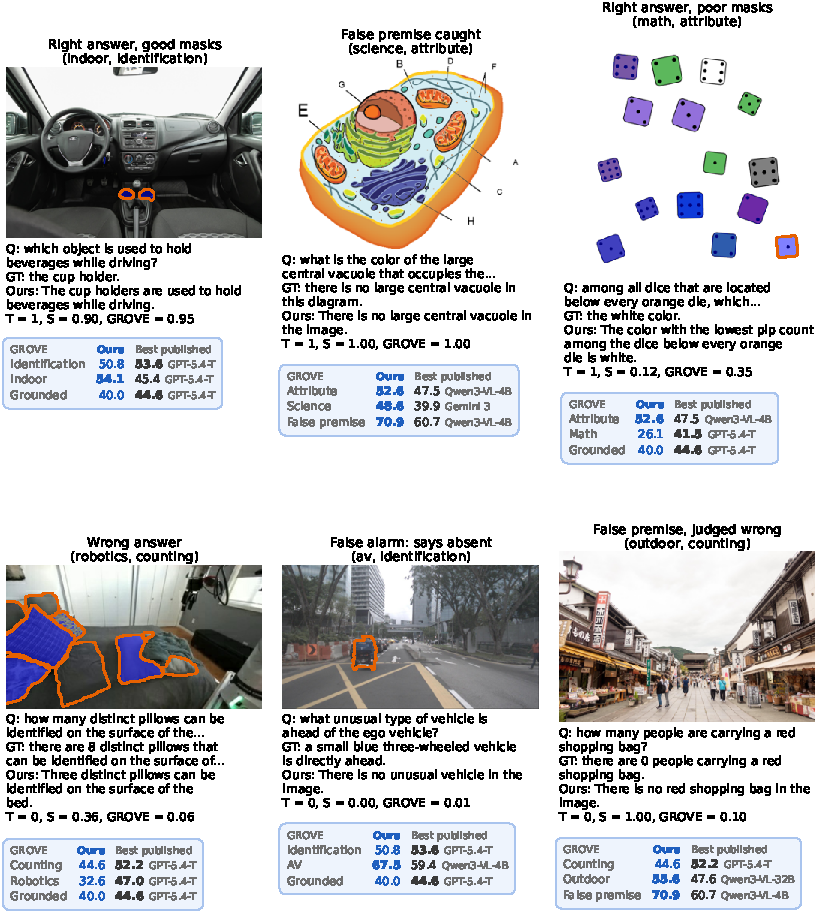
\includegraphics[width=\textwidth]{qual.pdf}
\caption{The entry on six VistaQA samples. Orange outline: ground-truth masks; blue fill: our masks. $T$: judge verdict
(AWQ), $S$: mask score. Blue boxes: our entry's GROVE (AWQ judge) next to the best published system's on the panel's task,
domain and question type (Table~\ref{tab:main}); the higher value is bold. Published per-sample outputs are not released, so the
comparison is by category, not by sample. Wrong answers include undercounting and premise false alarms on small objects; in the
last panel the judge rejects an answer that does reject the false premise. Images: VistaQA (CC BY 4.0).}
\label{fig:qual}
\end{figure}

\section{Breakdown of the entry}\label{app:anat}
All numbers here are aggregates of the entry's predictions and the official evaluator's per-sample output, computed after the
entry was frozen and scored. They describe the entry and changed nothing in it. We recover the per-sample mask score $S$ from the
per-sample GROVE $g$ and the verdict ($S=g^2$ if $T=1$, $S=(g/0.1)^2$ if $T=0$, and $S=0$ at the floor); the mean of the recovered
values reproduces the official mIoU of 52.05.

\textbf{Task by domain} (Table~\ref{tab:td}). Driving scenes are the best domain for five of the six tasks, and math or robotics is
the weakest for every task. The best cell is counting in driving scenes (79.9), the worst comparison in math (13.8).

\begin{table}[!htbp]
\centering\scriptsize
\caption{The entry's GROVE (AWQ judge) per task and domain ($n$ per cell 21--46; robotics has no OCR questions).}
\label{tab:td}
\begin{tabular}{lrrrrrrr}
\toprule
 & AV & Indoor & Outdoor & Science & Robotics & Math & All \\
\midrule
Identification & 66.4 & 60.7 & 61.9 & 44.2 & 41.0 & 23.3 & 50.8 \\
Attribute & 64.9 & 58.5 & 59.8 & 68.0 & 31.1 & 34.9 & 52.6 \\
OCR & 75.0 & 59.9 & 67.7 & 54.3 & -- & 19.2 & 58.4 \\
Spatial & 61.7 & 42.7 & 56.0 & 38.0 & 25.9 & 23.1 & 41.8 \\
Counting & 79.9 & 48.8 & 41.5 & 39.8 & 31.2 & 41.8 & 44.6 \\
Comparison & 60.2 & 51.6 & 46.0 & 47.5 & 33.0 & 13.8 & 43.2 \\
\midrule
\ours All & 67.5 & 54.1 & 55.6 & 48.6 & 32.6 & 26.1 & 48.4 \\
\bottomrule
\end{tabular}
\end{table}

\textbf{Where the points go} (Table~\ref{tab:loss}). Wrong answers on grounded questions cost 30.43 of the 51.60 points lost (59\%).
They are the largest item in every group, though only narrowly in science (3.95 against 3.82 for imperfect masks). Robotics loses the
most in total. Counting loses little to masks (0.61), because its right answers are few and have good masks (mean $S$ 73.8);
comparison is the reverse (2.98, mean $S$ 36.7).

\begin{table}[!htbp]
\centering\scriptsize
\setlength{\tabcolsep}{4pt}
\caption{The entry: where the points go. Number of samples, GROVE, text accuracy and mean $S$ on right grounded answers, then the GROVE
points lost (of 100), each as a share of the overall mean so that a block's rows add up. Grounded: wrong answer; right answer with
imperfect masks; right answer with no mask. False premise: wrong answer; right answer with masks. The instance-count block covers
grounded questions only.}
\label{tab:loss}
\begin{tabular}{lrrrrrrrrrr}
\toprule
 & & & & Mean & \multicolumn{3}{c}{Lost: grounded} & \multicolumn{2}{c}{Lost: false premise} & Total \\
Group & $n$ & GROVE & Text & $S$ & Wrong & Imperfect & No mask & Wrong & Masks & lost \\
\midrule
Identification & 214 & 50.8 & 60.3 & 66.7 & 5.52 & 1.78 & 0.23 & 1.57 & 0.00 & 9.11 \\
Attribute & 191 & 52.6 & 64.4 & 56.8 & 4.66 & 1.71 & 0.47 & 0.99 & 0.00 & 7.82 \\
OCR & 173 & 58.4 & 75.7 & 54.0 & 3.22 & 2.60 & 0.00 & 0.25 & 0.16 & 6.22 \\
Spatial & 199 & 41.8 & 56.3 & 46.9 & 5.43 & 2.27 & 0.16 & 1.85 & 0.31 & 10.02 \\
Counting & 188 & 44.6 & 47.9 & 73.8 & 7.02 & 0.61 & 0.23 & 1.07 & 0.08 & 9.01 \\
Comparison & 192 & 43.2 & 61.5 & 36.7 & 4.57 & 2.98 & 0.23 & 1.56 & 0.08 & 9.42 \\
\midrule
AV & 202 & 67.5 & 76.2 & 70.1 & 2.76 & 1.64 & 0.08 & 1.11 & 0.08 & 5.67 \\
Indoor & 205 & 54.1 & 65.9 & 58.3 & 4.52 & 2.00 & 0.23 & 1.22 & 0.16 & 8.13 \\
Outdoor & 196 & 55.6 & 68.4 & 58.2 & 4.46 & 1.91 & 0.39 & 0.68 & 0.08 & 7.51 \\
Science & 204 & 48.6 & 72.1 & 38.5 & 3.95 & 3.82 & 0.23 & 0.82 & 0.23 & 9.06 \\
Robotics & 200 & 32.6 & 40.5 & 51.5 & 7.84 & 1.41 & 0.23 & 2.17 & 0.00 & 11.65 \\
Math & 150 & 26.1 & 34.7 & 42.3 & 6.90 & 1.16 & 0.16 & 1.28 & 0.08 & 9.58 \\
\midrule
Single-instance & 596 & 43.1 & 62.8 & 53.1 & 18.50 & 9.80 & 1.01 & 0.00 & 0.00 & 29.32 \\
Multi-instance & 247 & 32.7 & 41.7 & 61.4 & 11.93 & 2.14 & 0.31 & 0.00 & 0.00 & 14.38 \\
\midrule
\ours All & 1157 & 48.4 & 60.8 & 54.9 & 30.43 & 11.94 & 1.32 & 7.28 & 0.62 & 51.60 \\
\bottomrule
\end{tabular}
\end{table}

\textbf{Answer against evidence.} On the 843 grounded questions, the entry has a right answer with good evidence ($S\geq0.5$) on
26.3\% and a wrong answer with weak evidence on 34.6\%. In 8.8\% the evidence is good but the answer wrong, and in 30.2\% the answer
is right but the evidence weak. Compared with answers and boxes alone (A + B), the premise check and the count raise move a net 63
samples into the wrong-and-weak group.

\textbf{Number of masks.} The entry predicts no mask for 383 samples; 314 have none in the ground truth. Of the 460 right grounded
answers with masks, 271 have the exact number (mean $S$ 0.74), 169 too many (0.33) and 20 too few (0.27). The excess sits on
single-instance questions: of those 361 answers, 200 are exact and 161 have too many. Of the 99 multi-instance ones, 71 are exact, 8
have too many and 20 too few.

\textbf{Premise check} (Table~\ref{tab:prem}). The 8B flags 707 of the 1,157 questions: 273 of 314 false-premise and 434 of 843
grounded. The yes/no confirmation keeps 335 of these (225 and 110), giving up 48 hits to remove 324 false alarms; the answer text
changes on 222 of the 225. Without the check, the 27B already denies the premise in 96 false-premise and 7 grounded answers. The check
gains on false-premise questions in every group and loses on grounded ones. Its net effect is negative for robotics, where it replaces
34\% of grounded answers, and for identification and counting. Of the 110 grounded answers it replaced, 63 had been right.

\begin{table}[!htbp]
\centering\scriptsize
\caption{Premise check of the entry per group: answers it changed among false-premise questions and among grounded ones (false alarms),
how many of the latter had been right, and the change in the group's GROVE from each side, against A + B.}
\label{tab:prem}
\begin{tabular}{lrrrrrr}
\toprule
Group & False premise changed & Grounded changed & Were right & $\Delta$ false premise & $\Delta$ grounded & Net \\
\midrule
AV & 53 / 63 (84\%) & 10 / 139 (7\%) & 6 & $+6.24$ & $-2.52$ & $+3.72$ \\
Indoor & 46 / 58 (79\%) & 9 / 147 (6\%) & 5 & $+8.43$ & $-1.34$ & $+7.09$ \\
Outdoor & 35 / 49 (71\%) & 19 / 147 (13\%) & 11 & $+5.51$ & $-3.92$ & $+1.59$ \\
Science & 48 / 60 (80\%) & 10 / 144 (7\%) & 7 & $+8.65$ & $-1.18$ & $+7.47$ \\
Robotics & 32 / 53 (60\%) & 50 / 147 (34\%) & 29 & $+8.73$ & $-9.56$ & $-0.83$ \\
Math & 8 / 31 (26\%) & 12 / 119 (10\%) & 5 & $+2.04$ & $-0.96$ & $+1.08$ \\
\midrule
Identification & 37 / 52 (71\%) & 29 / 162 (18\%) & 19 & $+4.88$ & $-6.44$ & $-1.56$ \\
Attribute & 43 / 55 (78\%) & 23 / 136 (17\%) & 14 & $+10.93$ & $-4.09$ & $+6.84$ \\
OCR & 30 / 45 (67\%) & 3 / 128 (2\%) & 1 & $+5.10$ & $-0.32$ & $+4.78$ \\
Spatial & 33 / 59 (56\%) & 24 / 140 (17\%) & 11 & $+7.01$ & $-2.64$ & $+4.37$ \\
Counting & 39 / 52 (75\%) & 15 / 136 (11\%) & 7 & $+1.77$ & $-2.35$ & $-0.58$ \\
Comparison & 40 / 51 (78\%) & 16 / 141 (11\%) & 11 & $+11.16$ & $-3.46$ & $+7.70$ \\
\midrule
\ours All & 222 / 314 (71\%) & 110 / 843 (13\%) & 63 & $+6.81$ & $-3.32$ & $+3.49$ \\
\bottomrule
\end{tabular}
\end{table}

\textbf{Count raise.} Of the 238 questions that match the count regex, 97 pass the plain-count guard. The rule raised 23 answers:
10 went from right to wrong, 2 from wrong to right, and 11 were wrong before and after. Eleven of the 23 lost their masks through the
bug described in Section~\ref{sec:results}.

\textbf{Image sizes} (image metadata only). The median image has 1.44\,MP and the largest 5.03\,MP. 536 of the 1,157 exceed the answerer's
1.64\,MP cap and are downscaled for the VLM only. Median per domain: driving 1600$\times$900 (0 of 202 above the cap); indoor and
outdoor 2250$\times$1500 (all 205 and 196); math 3.24\,MP (130 of 150); science 0.21\,MP (5 of 204); robotics 320$\times$180 (0 of 200).
Robotics images are therefore very small. We did not test upscaling them.

\section{Judge sensitivity and harness checks}\label{app:judge}
\textbf{Two builds of the judge.} Re-judging the entry's unchanged predictions with the unquantized model flips 56 of 1,157 verdicts
(4.8\%) and moves GROVE from 48.40 to 48.14 ($-0.26$, CI $-1.16$ to $+0.63$). Grounded questions gain (24 verdicts up, 10 down) and
false-premise questions lose (3 up, 19 down). Up / down by domain: driving 5/3, indoor 5/7, math 8/5, outdoor 4/1, robotics 2/8, science
3/5; by task: attribute 5/3, comparison 8/3, counting 1/7, identification 8/4, OCR 3/4, spatial 2/8. On proxy dev the two builds flip 8
of 560 verdicts (73.81 $\to$ 73.33); the full judge is stricter on OCR casing and near-synonyms. Under the full judge, v2, v3, v4 and
v5 trail the entry by 1.13, 0.85, 0.77 and 0.81, each with an interval that includes zero (for v2, $-3.01$ to $+0.79$), so neither
build separates them from the entry.

\textbf{Repeatability and quirks.} The same judge build is not perfectly repeatable: across two runs, 3 of 802 identical VistaQA
answers got a different verdict, which moved one analysis score by 0.06. The AWQ judge accepted 3 of 5 empty answers and the full
judge 2 of 5. These came from a first v5 run in which six large images failed (the premise override filled one answer); the six
fell back to the default input size before v5 was merged and judged. One false-premise answer that does reject the premise was judged wrong (Appendix~\ref{app:qual}, last panel).
Bootstrap intervals resample questions, so they do not include this judge noise.

\textbf{Harness checks,} made before any system was scored. Ground truth submitted as a prediction scores 100.00. Moving each answer
to the next sample while keeping the ground-truth masks gives 1.21\% text accuracy and GROVE 11.09, exactly what the formula
predicts: $100\,(0.0121 + 0.9879 \times 0.1)$. Re-running SAM2.1 on stored boxes reproduces 71.74 on proxy dev (548 of 560
predictions identical, the rest differing only numerically), and re-using stored verdicts reproduces a judged run exactly (73.05).

\textbf{Judge settings.} Official prompt and parser, temperature 0, at most 256 output tokens. The full judge ran in fp16 with a
1,024-token context (2,560 for v5, whose longest answer has 1,844 tokens).

\section{Development record}\label{app:dev}
Table~\ref{tab:sets} lists the dev sets and probes. Proxy dev and the premise, count and OCR probes decided the entry
(Table~\ref{tab:pre}), which reached 65.07 with answers and boxes, 72.27 with the premise check and 73.81 with the count raise. The
other sets came after the entry was scored and served only the analysis systems (Table~\ref{tab:post}). No number in these tables
comes from VistaQA. In proxy2, the driving-scene masks are SAM3 masks of annotated boxes, so those questions test which objects were
found rather than mask quality.

\begin{table}[!htbp]
\centering\scriptsize
\caption{Dev sets and probes. FP: false-premise questions. Masks: mean per grounded sample (VistaQA: 2.06). Probes have text ground truth only.}
\label{tab:sets}
\begin{tabular}{@{}>{\raggedright\arraybackslash}p{.72in}r>{\raggedright\arraybackslash}p{1.75in}rr>{\raggedright\arraybackslash}p{1.3in}@{}}
\toprule
Set & $n$ & Source & FP & Masks & Composition \\
\midrule
Proxy dev & 560 & COCO val2017, PACO-LVIS, COCO-Text v2; templated questions, answers and masks from annotations & 150 & 1.80 & counting 100, identification 70, spatial 70, comparison 60, attribute 60, OCR 50 \\
Proxy2 & 580 & Drawn charts and geometry, BOP (YCB-V, LM-O), 2018 Data Science Bowl, BDD100K & 158 & 4.08 & spatial 120, counting 116, attribute 107, comparison 101, identification 87, OCR 49; math 150, robotics 150, AV 150, science 130 \\
Proxy3 & 200 & RefCOCOg validation (UMD split), crowded scenes & 0 & 1.65 & spatial 140, comparison 60 \\
\midrule
Premise probe & 300 & MathVista testmini: 200 questions on their own image, 100 moved to another question's image & 100 & -- & false-alarm and recall check on figures \\
Count probe & 168 & MathVista testmini free-form integer questions matching the count regex & 0 & -- & count guard \\
OCR probe & 225 & TextVQA val reading questions, top answer with at least 5 of 10 votes & 0 & -- & OCR zoom; premise false alarms \\
Math probe & 200 & MathVista testmini & 0 & -- & thinking, calculator \\
V*Bench probe & 238 & V*Bench (SA-1B photos, median 3.38\,MP), with target boxes & 0 & -- & input resolution \\
WSP practice & 300 images & COCO val2017 outside proxy dev; each image with one absent-object and one present-object question & half & -- & Appendix~\ref{app:wsp} only \\
\bottomrule
\end{tabular}
\end{table}

\begin{table}[!htbp]
\centering\scriptsize
\caption{Decisions before the freeze, made on proxy dev and the three probes (GROVE / text accuracy unless stated; each chain as it
stood at the time). Shaded, at the bottom: the choices that make up the entry.}
\label{tab:pre}
\begin{tabular}{@{}>{\raggedright\arraybackslash}p{1.15in}>{\raggedright\arraybackslash}p{3.4in}>{\raggedright\arraybackslash}p{.6in}@{}}
\toprule
Decision & Measured & Outcome \\
\midrule
Premise on figures & Premise probe: 86 of 100 moved questions caught, 21 of 200 false alarms; OCR probe: 8 of 225 false alarms & No change \\
SAM3 veto of the premise check & $\tau$ 0.5--0.7: 73.16--73.18 vs 73.31 & Dropped \\
OCR zoom re-read & Proxy dev 73.96 (one net sample); OCR probe text 76.44 $\to$ 75.11 & Dropped \\
Thinking in the 27B & 73.64 vs 73.81 at three times the inference time; 34 of 560 traces unclosed & Dropped \\
Offline combinations & Concept masks on counting questions +0.05 to +0.16 (better and worse about equally often). Requiring the answers to agree with the premise check loses 43 hits to save 16 false alarms. Thinking against no-think: both right 432, both wrong 97, only one right 15 and 16, so no signal for a selector & None adopted \\
\midrule
\ours Answerer (one pass, SAM2.1-L) & Qwen3-VL-4B 39.02 / 55.7; Qwen3-VL-8B 58.60 / 66.4; Qwen3.5-9B 62.14 / 74.5; Qwen3.6-27B 64.91 / 71.2; Qwen3.6-35B-A3B not run (its fused experts stay unquantized in 4-bit loading) & 27B \\
\ours Two stages (reason, then ground each target) & 8B 58.56 / 65.0 against one pass 58.60 / 66.4; with an existence check 57.41 / 64.8; 4B two stages with the check 50.20 / 58.0 & One pass \\
\ours Short-answer rewrite & 8B 58.60 $\to$ 62.31 (296 of 560 answers had at most 3 words); 27B chain 71.74 $\to$ 72.29 & Kept \\
\ours Segmenter & SAM2.1-L 71.74, with multimask 71.53; SAM3 71.72; filled boxes for OCR: $S$ 0.649 vs SAM3 0.696 & SAM3 (also text-prompted) \\
\ours Premise checker & On the 27B's answers: 8B + confirm 71.74 (138 of 150 hits, 17 of 410 false alarms); the 27B's own check 69.60 (135, 36). 8B without confirm: 148, 105; reworded confirm: 133, 16; requiring both models: 73.39 vs 73.31 & 8B + confirm \\
\ours Count raise & SAM3 only at $\tau$ 0.7: 73.04; with the grammar fix 73.31; all three counters at $\tau$ 0.8: 73.81 (exact on 72 of 98 counting questions; the 27B alone 60) & Kept \\
\ours Count guard & Count probe, exact counts of 168: guarded 115, unguarded 108, no raise 114; judge text 75.60, 70.83, 75.00 & Guard kept \\
\bottomrule
\end{tabular}
\end{table}

\begin{table}[!htbp]
\centering\scriptsize
\caption{Tests after the freeze, decided on the dev sets only, in order (GROVE unless stated). Each rule was registered before its results.
Appendices~\ref{app:wsp}--\ref{app:ms} cover three more.}
\label{tab:post}
\begin{tabular}{@{}>{\raggedright\arraybackslash}p{1.15in}>{\raggedright\arraybackslash}p{3.4in}>{\raggedright\arraybackslash}p{.6in}@{}}
\toprule
Test & Measured & Outcome \\
\midrule
Qwen3.8-27B in the entry's chain & Proxy dev 74.70 vs 73.81 ($+0.89$, CI $-0.62$ to $+2.49$); proxy2 at the premise stage 61.04 vs 57.53 & v2 \\
Gemma 4 31B answerer & Proxy dev 69.77, text 79.5, mIoU 70.7, OCR 25.3 (its boxes come as $[y_1,x_1,y_2,x_2]$, swapped before SAM3) & No \\
Three-model majority & 316 of 410 grounded answers right; Qwen3.8 alone 320, oracle 338 & No \\
Evidence prompt naming the answer element & Everywhere on proxy2: 57.64 vs 57.42, but text 71.4 vs 73.8; math rises 68.0 $\to$ 78.0 & Figures only \\
Figure router & Yes on proxy dev 0 of 560; proxy2 math 150 of 150, science 2 of 130, driving and robotics 0 of 150; MathVista 199 of 200; TextVQA 11 of 225 & v2 \\
SAM3 veto $\tau$ & Pooled over proxy dev and proxy2: none 67.96; 0.7: 68.22; 0.6: 68.39; 0.5: 68.37; \textbf{0.4: 68.65}; 0.3: 68.45 & $\tau$ 0.4, v2 \\
Premise AND with Qwen3.8 & Proxy2 hits 139 of 158, false alarms 28 of 422 (8B alone 151, 39) & No \\
Thinking on all routed figures & MathVista 122 $\to$ 142 of 200; proxy2 65.42, below 65.87 & No \\
Reasoning router + thinking & MathVista 143 of 200; proxy2 65.87 & v3 \\
Thinking budget 8,192 tokens & Closes 10 of 18 unclosed traces, one more right answer & No \\
Answer selector (Qwen3.8 picks, Qwen3.6 unless overruled twice) & Proxy dev 65.46 (Qwen3.6 65.07, Qwen3.8 63.88, best-of-two ceiling 70.76); proxy2 56.85 (55.70, 60.04, 66.34); mostly position bias & No \\
Near-duplicate masks (IoU $\geq$ 0.5) & 11, 1, 1 and 0 masks dropped on four runs, changes of at most 0.01 & No \\
Three-way premise AND with veto & Proxy2 65.31 $\to$ 65.66; proxy dev 72.47 $\to$ 72.07 & No \\
Calculator tool & MathVista of 200: no thinking 122; always think 142; v3 recipe 143; tool instead of thinking 135; thinking, tool where the trace ran out 146; always the tool 140; proxy2 unchanged & Fallback, v4 \\
4\,MP input & V*Bench text 176 $\to$ 192 of 238, box hit 194 $\to$ 209 of 292 & v5 \\
Mask clean-up & Proxy dev / proxy2: hole filling $+0.43$ / $-0.05$; largest component $-1.30$ / $-0.16$; both $-0.85$ / $-0.21$ & No \\
\bottomrule
\end{tabular}
\end{table}

\section{Post-freeze systems v2--v5 (analysis, not the entry)}\label{app:v2}
The entry's aggregates (premise false alarms on 13\% of grounded questions, over-masking, weak math and robotics) prompted a
second system, built without looking at any VistaQA sample. Proxy dev is COCO-only, so we added \textbf{proxy2}: 580 questions
(158 false-premise) on drawn charts and geometry, BOP scenes~\cite{bop23} (YCB-V~\cite{posecnn}, LM-O~\cite{lmo}), 2018 Data
Science Bowl nuclei~\cite{dsb2018} and BDD100K~\cite{bdd100k}, with answers and masks from annotations or drawing code and
none of VistaQA's image sources. Each system below was chosen on the dev sets and registered before its one VistaQA run. Scores
in parentheses use the full judge.

\textbf{v2 did not transfer.} Each of its four changes won on the dev sets: (i) Qwen3.8-27B~\cite{qwen38} answers; (ii) a
Qwen3-VL-8B yes/no router sends charts, tables and diagrams to an evidence prompt that boxes the answer element (the bar, the
cell) instead of labels and legends; (iii) a SAM3 presence veto keeps the answer when SAM3 finds the object the premise check
calls missing (score $\geq 0.4$, picked by GROVE pooled over both dev sets); (iv) the count raise keeps masks. v2 gained 8.4 on
proxy2 and 0.4 on proxy dev but scored 48.01 (47.01), level with the entry ($-0.40$, 95\% CI $-2.38$ to $+1.55$; $-1.13$ with
the full judge). Stage by stage, the new backbone, +1.7 on proxy2, lost 3.0 on VistaQA at the answer stage (42.43 vs 45.46;
false-premise, math and science questions). The figure prompt, +2.6 on proxy2's drawn charts, gave nothing. With the veto,
``not present'' answers fell from 110 to 64 on grounded questions but also from 225 to 189 on false-premise ones, a small net
gain (+0.2 on v2; added to the entry with masks kept it gives 49.03, post hoc, not a submission). Keeping only the first mask on
non-counting answers, a registered test of the over-masking found in Section~\ref{sec:results}, scored 47.18.

\textbf{v3: thinking on multi-step questions.} Thinking on every routed figure raised MathVista probe accuracy from 61\% to 71\%
but lowered proxy2, whose figures ask for values read off a chart. A second yes/no router (does the question need several steps
of reasoning?) kept the gain (143/200) and left proxy2 unchanged; registered before v2 was scored, it became v3. On VistaQA it
sent 126 of the 353 figure questions to thinking: 22 answers turned right and 8 wrong (math 21.9 to 24.7), so v3 scored 48.21
(47.29), $+0.21$ over v2 (95\% CI $-0.35$ to $+0.75$) and level with the entry.

\textbf{v4: a calculator tool.} A larger thinking budget is no fix: 27 of v3's traces hit 4,096 tokens, and on the probe 8,192
closed 10 of 18 such traces but gained one answer. A calculator did better there: Qwen3.8 writes a short Python program that a
sandbox runs, raising the probe from 143 to 146 of 200. As v4 it ran on 21 of the 27 and changed 17 answers, 3 right gained and
3 lost: 48.37 (47.37), $+0.16$ over v3 (95\% CI $-0.23$ to $+0.56$), all of it judge flips on unchanged answers.

\textbf{v5: larger input images.} 536 VistaQA images exceed the answerer's 1.64\,MP cap (no dev image does), and on
V*Bench~\cite{vstar} (238 questions, 3.4\,MP photos) a 4.19\,MP cap gained 16 answers. As v5 it changed 156 answers on
VistaQA's large images, 22 right gained and 23 lost: 48.03 (47.34), level with v4.

The dev sets predicted the premise check's large gain but not the backbone or the figure prompt.
Appendix~\ref{app:transfer} compares dev-set and VistaQA effects for every change.

\section{Weight-space programming (analysis, not the entry)}\label{app:wsp}
After development closed we tested weight-space programming~\cite{takehi2026wsp}: a large LLM reads a small network's weights
and activations and writes new weights directly, without gradients. The editor was Claude Opus 5.5 (Anthropic), the coding
assistant that also wrote this pipeline; the edited model was Qwen3-VL-8B-Instruct. The target was its single-pass answers to
false-premise questions: on proxy dev they deny only 68 of 150 absent objects, while its own premise check (Pass C) catches 138.
Every edit decision used only a practice set built for it: 300 COCO val2017 images outside proxy dev, each with one question about
an absent, frequently co-occurring category and the same question about a present object (200 images for analysis, 100 for
scoring candidates).

At the first answer token, the absent-minus-present direction of the residual stream separates 97--99\% of question pairs from
layer 16 on, but only from layer 20 does it predict which absent objects the model denies (AUC 0.72 at layer 20, 0.87 at 24).
The edit chosen among 21 scored candidates (40 allowed) amplifies the layer-21 direction twofold in what layers 18--20 write
(rank-1 updates of their six output projections, centred by a bias) and adds a bias on layer 20 that moves the residual 0.3
class gaps towards ``absent''. On the scoring images, denials rose from 75 to 85 of 100 absent objects and from 4 to 5 of 100
present ones. The selection rules and the paired VistaQA runs were registered first, then the edit itself, all before any
dev-set run.

\textbf{Result.} With SAM3 box masks, the edit raised the 8B's single-pass GROVE from 53.30 to 55.86 on proxy dev and proxy2
pooled ($+2.57$, CI $+1.71$ to $+3.50$), and from 38.76 to 40.46 on VistaQA ($+1.70$, CI $+0.83$ to $+2.60$). On VistaQA it changed
154 answers, with 27 verdicts gained and 8 lost: false-premise GROVE rose from 39.7 to 45.5, and grounded GROVE stayed level (38.4
to 38.6). That is about 30\% of what the 8B premise check adds (44.35 for the unedited model with the check), at no extra inference
cost. On top of the check, the edit adds nothing significant ($+0.56$, CI $-0.02$ to $+1.18$). The entry takes its answers from the
27B, so it is unaffected.

\section{Mask verifier (analysis, not the entry)}\label{app:mv}
After development closed we also tested a training-free fix for the over-masking of Section~\ref{sec:results}, registered before
any of its results. For each prediction with at least two masks on a non-counting question, a Set-of-Mark check~\cite{yang2023som}
draws each mask's bounding box with its number on the image and asks a VLM which numbered boxes mark ``visual evidence required to
support this answer'' (VistaQA's definition), with the question and the answer in the prompt and a JSON list as the reply. Masks it
does not list are dropped; without a valid list, all are kept. Answers never change, so the text verdicts are reused. We compared
two checkers: the answerer (Qwen3.6-27B) and Qwen3-VL-8B.

Proxy dev and proxy2 hold few over-masked answers, so we built \textbf{proxy3}: 200 questions on RefCOCOg~\cite{mao2016refcocog}
validation images (UMD split~\cite{nagaraja2016refcocog}), which hold several objects of one category. Each question names its
objects by a referring expression: which side of the image, left or right of another object, or which appears larger. The entry's
answer and mask passes over-mask 19 of their 179 right grounded answers there.

\textbf{Result.} On the three dev sets pooled (1,340 questions), the 27B checker beat the 8B, which lost 0.65, but still scored
below no check at all: 66.96 against 67.34 ($-0.38$, CI $-0.63$ to $-0.15$). It fixed 15 of 49 over-masked answers, but 32 of the 72
predictions it changed already had the right number of masks; in 26 of them it kept only one of the two objects in ``Which appears
larger, the A or the B?'' or ``Is the A left or right of the B?''. On VistaQA, run as registered, it dropped 111 masks from 98
predictions. Over-masked right answers fell from 169 to 140, 8 drops hit a correct count, and mIoU rose from 52.05 to 52.50. GROVE
moved from 48.40 to 48.61 ($+0.21$, CI $-0.13$ to $+0.53$), which is not significant. Over-masking is rare on the dev sets (6\% of
right grounded answers with masks, against 37\% on VistaQA), which is why they predicted a loss. The entry is unchanged.

\section{Model swaps (analysis, not the entry)}\label{app:ms}
After development closed we tested two model swaps in the entry's chain, each alone and registered before any of their results:
Qwen3-VL-32B-Instruct~\cite{qwen3vl} as the answerer in place of Qwen3.6-27B, and Gemma~4 31B (instruction-tuned)
as the premise checker in place of Qwen3-VL-8B. Both ran in 4-bit like the 27B, with the entry's prompts; every other pass and
rule is unchanged. Proxy3 (Appendix~\ref{app:mv}) has no false premises, so every premise override there is a false alarm.

\textbf{On the dev sets} (1,340 questions pooled), the entry's chain scores 66.27; it includes the premise check on proxy3, so this
differs from the mask verifier's base. The 32B answerer was level with it at 66.32 ($+0.05$, CI $-1.27$ to $+1.42$): it lost 2.0 on
proxy dev (COCO) and gained 1.4 on proxy2 and 1.9 on proxy3. Gemma turned about as many false-premise answers into ``not present''
as the 8B (105 vs 106 of 150 on proxy dev, 117 vs 121 of 158 on proxy2) but raised more false alarms on grounded questions (35 vs 17
of 410 on proxy dev, 31 vs 22 of 200 on proxy3; 33 vs 39 of 422 on proxy2), and scored 64.47 ($-1.80$, CI $-3.11$ to $-0.50$).

\textbf{On VistaQA}, run as registered, the ranking reversed. Gemma changed 239 of 314 false-premise answers (the 8B: 222) and 120 of
843 grounded ones (the 8B: 110). False-premise GROVE rose from 70.9 to 78.6 and grounded GROVE fell from 40.0 to 39.0, for 49.76
overall: $+1.35$ (CI $-0.20$ to $+2.93$), not significant. The 32B scored 43.38, a loss of 5.02 (CI $-6.92$ to $-3.15$). Its text
accuracy fell from 60.8 to 58.4 and mIoU from 52.1 to 47.3, most of all on driving scenes, where GROVE fell from 67.5 to 45.8 while
text accuracy fell only from 76.2 to 73.8. Proxy2's BDD100K questions did not show this. The entry is unchanged.

\textbf{The driving-scene loss is in the masks}, not the answers. Mean $S$ on right grounded answers fell from 70.1 to 26.2 on driving
scenes and moved by at most 2.3 in the other domains, with similar mask counts; driving scenes account for about 3.8 of the 5.02
points lost. On their 1600$\times$900 images, the 32B's single boxes have median ratios to the 27B's of 0.95 (x-centre), 0.97
(y-centre), 0.95 (width) and 0.88 (height), with $n=76$. In the other domains the ratios are about 1.00, and on proxy2's
1280$\times$720 BDD100K images the centre ratios are 1.00 ($n=54$). Published Qwen3-VL-32B + SAM3 scores 58.40 on driving scenes, so
this looks like a coordinate shift at that image size in our 4-bit run, not a limit of the model. Our registered rule allows re-runs
only for infrastructure failures, so we did not re-run it.

\section{How dev-set effects carried over to VistaQA}\label{app:transfer}
Table~\ref{tab:transfer} puts each change's effect on the dev sets beside its effect on VistaQA, paired on the same samples. The dev
sets gave the right sign in 5 of 12 rows. The correlation between pooled dev effects and VistaQA effects is 0.23 (Pearson) and 0.08
(Spearman); the rows share systems and samples, so these numbers are descriptive only. Only two changes have intervals that exclude
zero with the same sign on both sides: the premise check and the weight edit. The largest dev gains, the whole of v2 and the figure
router, came to nothing, and the 32B answerer's level dev result hid a large loss. Proxy3 has no false-premise questions, so the premise
check can only lose there.

Three more changes were decided on text-only probes, so they have no dev GROVE: thinking on reasoning questions (MathVista 122 $\to$
143 of 200; VistaQA v3 $+0.21$ over v2), the calculator (143 $\to$ 146; v4 $+0.16$ over v3) and 4\,MP input (V*Bench 176 $\to$ 192 of
238; v5 $-0.34$ against v4). None of the three VistaQA differences is significant.

Table~\ref{tab:across} shows the entry's chain on each set. VistaQA is harder than every dev set on every task and on both question
types. On false-premise questions the gap is about 21 points (70.9 against 91.5 and 92.2): the premise check catches 92\% and 96\% of
them on proxy dev and proxy2 and 71\% on VistaQA, so the dev sets overstated its recall.

\begin{table}[!htbp]
\centering\scriptsize
\setlength{\tabcolsep}{3pt}
\caption{Effect of each change in GROVE (AWQ judge). Columns 2--4 are point differences per dev set; pooled and VistaQA give paired
bootstrap 95\% CIs; the last column says whether the signs agree. Pooled uses the sets with a value in that row. Shaded, at the
bottom: the entry's two stages.}
\label{tab:transfer}
\begin{tabular}{lrrrllc}
\toprule
Change & Proxy dev & Proxy2 & Proxy3 & Dev, pooled & VistaQA & Sign \\
\midrule
Count raise keeps masks & -- & $+0.80$ & -- & $+0.80$ [$+0.29$, $+1.43$] & $+0.07$ [$+0.00$, $+0.17$] & yes \\
Qwen3.8 for Qwen3.6, answer stage & $-1.19$ & $+1.72$ & -- & $+0.29$ [$-1.61$, $+2.17$] & $-3.04$ [$-5.26$, $-0.84$] & no \\
Figure router, element evidence & -- & $+2.62$ & -- & $+2.62$ [$+1.20$, $+4.09$] & $-0.24$ [$-0.89$, $+0.37$] & no \\
SAM3 veto ($\tau$ 0.4) & $-0.32$ & $+1.67$ & -- & $+0.70$ [$-0.12$, $+1.52$] & $+0.22$ [$-0.72$, $+1.15$] & yes \\
Whole of v2 vs the entry & $+0.42$ & $+8.44$ & -- & $+4.50$ [$+2.96$, $+6.07$] & $-0.40$ [$-2.38$, $+1.55$] & no \\
Weight edit of the 8B & $+3.24$ & $+1.92$ & -- & $+2.57$ [$+1.71$, $+3.50$] & $+1.70$ [$+0.83$, $+2.60$] & yes \\
Weight edit, both with premise check & $+0.43$ & $+0.13$ & -- & $+0.28$ [$-0.03$, $+0.62$] & $+0.56$ [$-0.02$, $+1.18$] & yes \\
Set-of-Mark mask check & $-0.48$ & $-0.38$ & $-0.10$ & $-0.38$ [$-0.63$, $-0.15$] & $+0.21$ [$-0.13$, $+0.53$] & no \\
Qwen3-VL-32B answerer & $-2.01$ & $+1.42$ & $+1.87$ & $+0.05$ [$-1.27$, $+1.42$] & $-5.02$ [$-6.92$, $-3.15$] & no \\
Gemma 4 31B premise check & $-2.19$ & $-0.73$ & $-3.82$ & $-1.80$ [$-3.11$, $-0.50$] & $+1.35$ [$-0.20$, $+2.93$] & no \\
\midrule
\ours Premise check (8B) & $+7.20$ & $+1.83$ & $-7.17$ & $+2.73$ [$+1.03$, $+4.45$] & $+3.49$ [$+1.65$, $+5.35$] & yes \\
\ours Count raise & $+1.54$ & $-0.10$ & -- & $+0.71$ [$+0.02$, $+1.41$] & $-0.55$ [$-1.02$, $-0.13$] & no \\
\bottomrule
\end{tabular}
\end{table}

\begin{table}[!htbp]
\centering\scriptsize
\caption{The entry's chain on each set: GROVE per task and question type, then text accuracy, mIoU and overall GROVE. Proxy3 has
only spatial and comparison questions and no false premises; with no counting questions, its chain ends at the premise check.
VistaQA shaded.}
\label{tab:across}
\begin{tabular}{lrrrrrrrrrrr}
\toprule
Set & Ident. & Attr. & OCR & Spat. & Count & Comp. & FP & Gr. & Text & mIoU & GROVE \\
\midrule
Proxy dev (560) & 68.2 & 63.5 & 59.8 & 73.1 & 65.7 & 72.5 & 91.5 & 67.3 & 79.8 & 76.5 & 73.81 \\
Proxy2 (580) & 54.2 & 71.0 & 75.4 & 54.8 & 46.0 & 53.4 & 92.2 & 44.4 & 75.5 & 56.9 & 57.43 \\
Proxy3 (200) & -- & -- & -- & 73.3 & -- & 65.0 & -- & 70.8 & 81.5 & 67.7 & 70.78 \\
\midrule
\ours VistaQA (1,157) & 50.8 & 52.6 & 58.4 & 41.8 & 44.6 & 43.2 & 70.9 & 40.0 & 60.8 & 52.1 & 48.40 \\
\bottomrule
\end{tabular}
\end{table}

\end{document}
